\documentclass[conference]{IEEEtran}
\usepackage{newtxtext}
\IEEEoverridecommandlockouts
\usepackage{cite}
\usepackage{amsmath,amssymb,amsfonts}
\usepackage{algorithmic}
\usepackage{graphicx}
\usepackage{textcomp}
\usepackage{xcolor}
\usepackage{booktabs}
\usepackage{multirow}
\usepackage{url}
\usepackage{listings}
\usepackage{tikz}
\usepackage{pgfplots}
\pgfplotsset{compat=1.18}

\usetikzlibrary{shapes.geometric, arrows.meta, positioning, fit, backgrounds}

\lstset{
  basicstyle=\footnotesize\ttfamily,
  frame=none,
  breaklines=true,
  columns=fullflexible,
  keepspaces=true,
  captionpos=b
}

\begin{document}

\title{From Brownfield CLI to Intent Models: A Guardrailed Agentic Translation Workflow}

\author{
\IEEEauthorblockN{Navin Suvarna}
\IEEEauthorblockA{Independent Researcher\\
Holly Springs, NC, USA\\
nsuvarna@cisco.com\\
0009-0004-0161-2372}
\and
\IEEEauthorblockN{Karthik Pappu}
\IEEEauthorblockA{Dakota State University\\
Madison, SD, USA\\
karthik.pappu@trojans.dsu.edu\\
0009-0000-5335-6279}
\and
\IEEEauthorblockN{Saurabh Sharma}
\IEEEauthorblockA{Independent Researcher\\
Apex, NC, USA\\
saurabh.sharma24@gmail.com\\
0009-0001-5486-8062}
\and
\IEEEauthorblockN{Belete Ageze}
\IEEEauthorblockA{Independent Researcher\\
Ellicott City, MD, USA\\
bageze@cisco.com\\
0009-0007-4510-8815}
}

\maketitle

\begin{abstract}
Adopting intent-based controllers requires migrating brownfield CLI (command-line interface) configurations to intent models. Manual translation is impractical; LLM (large language model) outputs are schema-valid yet semantically wrong without guardrails. Our hybrid deterministic-agentic workflow translates brownfield switching configurations into validated YAML (YAML Ain't Markup Language) intent objects. Vendor-aware routing sends IOS-XE and EOS through deterministic parsers; LLM fallback handles unsupported platforms and validator-driven retry. A two-tier validator enforces schema and 22 semantic rules with feedback-driven retry and human escalation. We evaluate on 97 sanitized campus switching configurations (six roles) via a four-approach controlled ablation: (RQ1) does the hybrid workflow improve correctness over deterministic and zero-guardrail LLM baselines; (RQ2) is semantic validity orthogonal to schema compliance and reduced by guardrails; (RQ3) does the workflow surface ambiguity for retry or escalation rather than silent acceptance. Approach~B+ (schema-constrained LLM) reaches 85.6\% schema yet 0.0\% semantic validity at 26.3~s, separating schema and semantic correctness as failure modes (RQ2). Approach~C reaches 99.0\% semantic validity at 115~ms median, F1\,=\,0.921 (RQ1); the 99.0-pp B+$\to$C gap is consistent with the guardrail layer (normalizer + 22 rules + retry) as primary contributor in this ablation. Stress tests confirm escalation on degraded inputs (RQ3).
\end{abstract}

\begin{IEEEkeywords}
intent-based networking, network automation, brownfield migration, configuration translation, guardrailed agentic workflow, semantic validation, configuration mapping ambiguity taxonomy, LangGraph, retrieval-augmented generation, Cisco IOS-XE, Arista EOS
\end{IEEEkeywords}

\section{Introduction}

\subsection{Problem Statement}

Enterprise campus networks accumulate device configurations over years of incremental change. These \emph{brownfield} configurations are expressed as vendor-specific CLI artifacts: thousands of lines of IOS-XE or EOS syntax encoding Virtual Local Area Networks (VLANs), Virtual Routing and Forwarding (VRF) instances, Access Control Lists (ACLs), 802.1X policy, and uplink topology that have never been captured in a machine-readable intent model~\cite{martinez2015cli}. When an organization adopts an intent-based network controller, the controller requires structured YAML intent objects aligned to its data model before it can manage existing devices~\cite{leivadeas2023survey,juniper2023apstra}. Producing these objects by hand from raw CLI output is the dominant bottleneck in brownfield migration projects.

Two common automation strategies both fall short in practice. A purely deterministic approach handles unambiguous cases well but breaks on configurations containing contextual or semantic ambiguity; for instance, an interface whose role (access versus routed uplink) cannot be determined from syntax alone. A zero-guardrail LLM approach improves coverage but generates outputs that are syntactically plausible yet structurally or semantically incorrect without constrained generation and post-hoc validation~\cite{wu2024netllm,dzeparoska2023policy,ji2023survey}. Neither approach provides the auditability, confidence scoring, or human escalation path required for production adoption. A less-recognized failure mode underlies both: \emph{semantic validity is orthogonal to both syntactic parsing correctness and schema compliance}. An intent object can satisfy a strict YAML schema and still be semantically broken; for example, referencing an ACL in an SNMP community restriction that does not exist in the extracted ACL table. This cross-reference class of error is invisible to schema validators and to field-level parsers alike, and neither purely deterministic nor LLM approaches detect it without an explicit semantic rule engine. The evaluation demonstrates this concretely: the schema-constrained LLM baseline (Approach~B+) achieves \emph{worse} schema and semantic validity than the zero-guardrail LLM; prompt engineering cannot close the semantic gap.

\subsection{Research Questions}

This study is organized around three research questions:

\textbf{RQ1:} How does a hybrid deterministic-agentic guardrailed workflow affect translation correctness and completeness relative to purely deterministic and zero-guardrail LLM baselines?

\textbf{RQ2:} Is semantic validity a failure mode orthogonal to schema compliance, and do semantic guardrails materially reduce schema-valid but semantically incorrect intent outputs that neither syntactic parsers nor LLM prompting detect?

\textbf{RQ3:} How does the workflow expose ambiguity, validation failures, and unsupported-platform mappings for retry or human escalation rather than silent acceptance?

\subsection{Contributions}


\textbf{Hybrid Workflow for Brownfield Intent Translation:} A staged brownfield translation workflow with deterministic parsing, selective LLM-assisted mapping, schema validation, semantic rule guardrails, and exception handling, implemented as a LangGraph state machine with vendor-specific routing. The deterministic path is validated on all 97 production-derived configurations spanning six deployment roles; the LLM fallback path is validated across five routing/escalation stress cases and 15 real Cisco NX-OS (Nexus OS) configurations spanning eight roles (100\% schema and semantic validity; macro-F1\,=\,0.217).

\textbf{Configuration Mapping Ambiguity Taxonomy (CMAT):} A four-class taxonomy (deterministic, contextual, semantic, indeterminate) with a routing policy that assigns each class to the appropriate pipeline stage. Each class has direct empirical coverage: deterministic fields drive the 97-config corpus at 115~ms with no LLM calls; contextual fields route to the LLM fallback (15 real NX-OS configs); semantic fields are handled by the 22-rule engine (accounting for the 99.0 percentage-point (pp) B+$\to$C gap); indeterminate fields escalate to human review (confirmed in five stress cases). CMAT is designed to generalize beyond any specific controller schema.

\textbf{Empirical Isolation of the Semantic Validity Gap:} A four-approach controlled ablation on 97 sanitized campus switching configs showing schema validity and semantic validity are orthogonal. Schema injection (Approach~B+) worsens both schema and semantic correctness relative to the unconstrained LLM baseline; the B+$\to$C gap (99.0~pp) isolates the guardrail contribution as the mechanism responsible for semantic validity improvement in this ablation.


\section{Related Work}

\textbf{Intent-based networking:} Intent-based networking (IBN)~\cite{clemm2022ibn} systems such as commercial campus network controllers~\cite{leivadeas2023survey} and Apstra~\cite{juniper2023apstra} manage network state through high-level declarative models built on the programmable network paradigm~\cite{kreutz2015sdn}. YANG (Yet Another Next Generation data modeling language)~\cite{bjorklund2010yang}, OpenConfig~\cite{openconfig2016}, NETCONF (Network Configuration Protocol)~\cite{enns2011netconf}, and RESTCONF (REST-based NETCONF)~\cite{bierman2017restconf} provide model-driven interfaces for configuration and telemetry. Translating legacy CLI into such models remains an open operational challenge~\cite{leivadeas2023survey}.

\textbf{Configuration verification:} Tools such as Header Space Analysis~\cite{kazemian2012hsa}, Batfish~\cite{fogel2015batfish}, Minesweeper~\cite{beckett2017minesweeper}, and NetDice~\cite{steffen2020netdice} verify semantic properties of existing configurations and inform our semantic rule categories, though they address errors in deployed configs, not mapping correctness of generated intent objects, the gap this paper targets.

\textbf{LLMs for networking:} Prior LLM work targets networking task adaptation~\cite{wu2024netllm}, policy translation from natural language~\cite{dzeparoska2023policy}, and spec$\to$config synthesis~\cite{mondal2023router} (inverse of brownfield CLI$\to$intent). None enforce semantic postconditions inline. The directly comparable threads, namely LLM-only translation~\cite{mondal2023router} and constrained decoding~\cite{scholak2021picard}, are evaluated as Approaches~B and B+ in this paper's ablation.

\textbf{Constrained and guardrailed generation:} Structured output techniques~\cite{willard2023guided} and prompt-based constraint injection~\cite{beurerkellner2023prompting} improve LLM output regularity; constrained decoding for structured targets such as SQL has been studied in~\cite{scholak2021picard}. Our work applies retrieval-augmented generation (RAG) context injection~\cite{lewis2020rag,gao2023rag} to constrain mapper output to a specific intent schema, and supplements this with a post-generation rule engine rather than relying on the LLM to self-validate.

\textbf{Workflow orchestration:} The reasoning-and-acting paradigm~\cite{yao2023react} underpins modern agentic workflows; LangGraph~\cite{langchain2024langgraph} and similar orchestration frameworks~\cite{wu2023autogen} realize this as modular multi-step pipelines with conditional branching. Our contribution is the networking-specific orchestration policy and validation pipeline built on top of these primitives, not the framework itself.

\textbf{Brownfield migration:} Industry uses manual inspection and proprietary migration wizards bundled with controllers~\cite{leivadeas2023survey,juniper2023apstra}; these are vendor-coupled and not benchmarked openly. Academic CLI abstraction~\cite{martinez2015cli} parses but does not normalize or validate against a controller schema. This work differs on three axes: hybrid deterministic-first routing with explicit ambiguity classification, a rule engine separating schema from semantic validity with quantified gap, and reported escalation rate with structured exception reports.

\section{System Model and Problem Formulation}

\textbf{Task:} Let $C$ denote a raw device configuration as unstructured CLI text. Translation is a function $T: C \rightarrow I$ where $I$ conforms to target schema $\mathcal{S}$. Three difficulty classes arise: \emph{structural complexity} (thousands of interface stanzas and ACL entries), \emph{referential integrity} (cross-references among VRFs, VLANs, RADIUS servers, and Authentication, Authorization, and Accounting (AAA) groups must remain consistent), and \emph{semantic validity} (a schema-valid $I$ may still be semantically wrong, e.g.\ a routing-adjacency interface mapped to access-edge intent).

\textbf{Scope:} (i)~campus switching platforms (Cisco Catalyst 3850/9300/9500; Arista EOS access-distribution); (ii)~target is a commercial controller YAML intent schema (eleven template categories); (iii)~ground-truth intent objects available; (iv)~credential handling and device-side commits out of scope.

\textbf{Pipeline and CMAT routing:} Eight stages: \emph{parse $\rightarrow$ vendor-route $\rightarrow$ map $\rightarrow$ normalize $\rightarrow$ validate $\rightarrow$ semantic-check $\rightarrow$ generate $\rightarrow$ report}. Stages 1--4 are purely deterministic for IOS-XE/EOS; the LLM is invoked only on unsupported-platform fallback or validator-driven retry. Routing follows the \textbf{Configuration Mapping Ambiguity Taxonomy (CMAT)} with four mutually exclusive classes: deterministic (syntactic map), contextual (LLM+RAG), semantic (rule engine), and indeterminate (human review). No prior taxonomy partitions CLI translation by routing-policy implication.

\textbf{Metrics:} Field-level accuracy (macro-F1 over (field-path, value) pairs), object completeness (fraction of GT top-level blocks present), schema validity rate, semantic validity rate (fraction passing all 22 rules), escalation rate (configs routed to human review after retries). \emph{Primary endpoint}: field-level macro-F1 (RQ1); \emph{co-primary}: semantic validity rate (RQ2); schema validity, escalation rate, and latency are secondary. \emph{Comparison plan}: per-approach differences are reported as observed point gaps; no inferential test is performed because deterministic paths produce bit-identical output across runs (computational details in §\ref{sec:results}). Human correction time and unsupported-mapping detection require live deployment and are deferred (§\ref{sec:stress} provides qualitative escalation evidence).

\textbf{Hypotheses:} \textbf{H1}: hybrid workflow improves correctness/completeness over deterministic-only and zero-guardrail LLM baselines on configurations with contextual or semantic ambiguity. \textbf{H2}: schema validation alone is insufficient; semantic guardrails reduce schema-valid but semantically invalid outputs. \textbf{H3}: unsupported or degraded inputs route to retry or human escalation rather than silent acceptance.

\section{Experimental Methodology}

\subsection{Prototype Architecture}

The pipeline is implemented as a LangGraph~\cite{langchain2024langgraph} state machine; each processing stage is a node in the graph and edges implement deterministic routing and conditional retry logic. The shared state object (\texttt{AgentState}) carries the raw configuration, intermediate representations (\texttt{legacy\_parsed\_data}, \texttt{extracted\_intent}, \texttt{normalized\_intent}), validation results with confidence scores, and a trace log consumed by the Reporter.

Figure~\ref{fig:workflow} illustrates the pipeline with its vendor-aware branching and retry path.

\begin{figure*}[!t]
\centering
\resizebox{0.94\textwidth}{!}{%
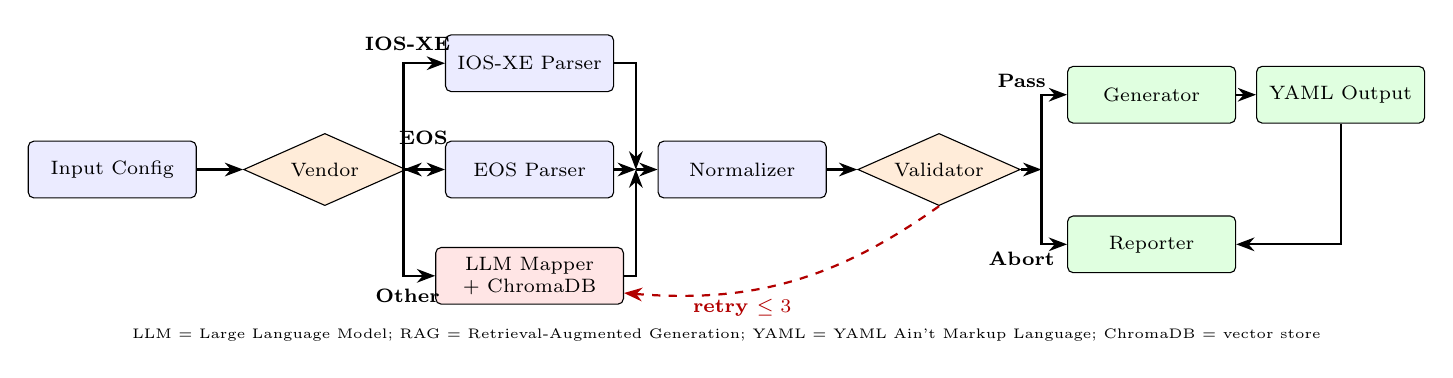
\begin{tikzpicture}[
  font=\scriptsize,
  box/.style={rectangle, draw, rounded corners=2pt, fill=blue!8,
              text centered, minimum height=0.72cm, text width=1.9cm},
  decision/.style={diamond, draw, fill=orange!15, text centered,
                   inner sep=1pt, text width=1.45cm, aspect=2.25},
  llmbox/.style={rectangle, draw, rounded corners=2pt, fill=red!10,
                 text centered, minimum height=0.72cm, text width=2.15cm},
  termbox/.style={rectangle, draw, rounded corners=2pt, fill=green!12,
                  text centered, minimum height=0.72cm, text width=1.9cm},
  arr/.style={-Stealth, thick},
  retarr/.style={-Stealth, thick, dashed, red!70!black}
]

% Nodes
\node[box]      (input)  at (0,0)       {Input Config};
\node[decision] (router) at (2.7,0)     {Vendor};

\node[box]      (cisco)  at (5.3,1.35)  {IOS-XE Parser};
\node[box]      (eos)    at (5.3,0)     {EOS Parser};
\node[llmbox]   (llm)    at (5.3,-1.35) {LLM Mapper\\+ ChromaDB};

\node[box]      (norm)   at (8.0,0)     {Normalizer};
\node[decision] (val)    at (10.5,0)    {Validator};

\node[termbox]  (gen)    at (13.2,0.95) {Generator};
\node[termbox]  (rep)    at (13.2,-0.95){Reporter};
\node[termbox]  (out)    at (15.6,0.95) {YAML Output};

% Helper coordinates
\coordinate (rout) at (3.7,0);
\coordinate (merge) at (6.65,0);
\coordinate (vout) at (11.8,0);

% Input to router
\draw[arr] (input.east) -- (router.west);

% Router split
\draw[arr] (router.east) -- (rout);
\draw[arr] (rout) |- (cisco.west);
\draw[arr] (rout) -- (eos.west);
\draw[arr] (rout) |- (llm.west);

% Clean fixed branch labels
\node[font=\scriptsize\bfseries] at (3.75,1.6) {IOS-XE};
\node[font=\scriptsize\bfseries] at (3.95,0.40) {EOS};
\node[font=\scriptsize\bfseries] at (3.75,-1.6) {Other};

% Parser merge
\draw[arr] (cisco.east) -| (merge);
\draw[arr] (eos.east) -- (merge);
\draw[arr] (llm.east) -| (merge);
\draw[arr] (merge) -- (norm.west);

% Normalizer to validator
\draw[arr] (norm.east) -- (val.west);

% Validator split
\draw[arr] (val.east) -- (vout);
\draw[arr] (vout) |- (gen.west);
\draw[arr] (vout) |- (rep.west);

% Clean fixed validator labels
\node[font=\scriptsize\bfseries] at (11.55,1.13) {Pass};
\node[font=\scriptsize\bfseries] at (11.55,-1.13) {Abort};

% Output and report path
\draw[arr] (gen.east) -- (out.west);
\draw[arr] (out.south) |- (rep.east);

% Retry path, isolated below the diagram
\draw[retarr] (val.south) to[bend left=20] (llm);
\node[font=\scriptsize\bfseries, red!70!black] at (8.0,-1.75) {retry $\leq 3$};

% Compact on-figure abbreviation key
\node[font=\tiny, align=center] at (7.8,-2.10)
  {LLM = Large Language Model; RAG = Retrieval-Augmented Generation; YAML = YAML Ain't Markup Language; ChromaDB = vector store};

\end{tikzpicture}%
}
\caption{LangGraph pipeline with vendor-aware routing and validator retry loop. Orange diamonds = decision nodes (Vendor router, Validator); blue rectangles = deterministic processing stages (IOS-XE/EOS parsers, Normalizer); red rectangle = LLM Mapper (LLM = Large Language Model) augmented with retrieval-augmented generation (RAG) from a ChromaDB vector store indexed on the target intent schema, invoked only for unsupported-vendor inputs and validator-driven retry; green rectangles = terminal stages (Generator, Reporter, YAML Output, where YAML = YAML Ain't Markup Language). The dashed red arrow marks the validator-triggered feedback path back to the LLM Mapper, capped at three retry iterations before the workflow aborts to a structured escalation report (``Abort'' branch on Validator).}
\label{fig:workflow}
\end{figure*}

\subsection{Implementation Stack}

Vendor-specific Python parsers (\texttt{cisco\_parser.py} for IOS-XE, \texttt{arista\_parser.py} for EOS) implement approximately 20 regex-based extraction methods per vendor, covering interfaces, VLANs, VRF instances, ACLs, Remote Authentication Dial-In User Service (RADIUS) servers, 802.1X bindings, storm-control, NTP, DNS, Simple Network Management Protocol (SNMP), and banners; the parsing stage invokes no LLM. When the LLM path is activated (unsupported platforms or post-validation retry), OpenAI \texttt{gpt-4.1-mini} is queried at temperature~0.1; retrieved context from a ChromaDB vector store (indexed on the target intent schema and Jinja2 template variable schemas via \texttt{text-embedding-3-large} embeddings, top-3 retrieval) is injected into the mapper prompt to constrain field names, types, and nesting. Token optimization strips routing-protocol blocks and deduplicates interface definitions before invocation.

A deterministic normalizer post-processes all mapper outputs regardless of path, promoting nested LLM-generated fields to root-level keys, normalizing IP address representation, and converting flat interface lists to typed \texttt{access\_interfaces} and \texttt{routed\_interfaces} collections. The validation rule engine loads rules from \texttt{validation/rules/*.py}, enforces required fields, object types, enumerations, nesting, and referential consistency, and computes a confidence score from 0.0 to 1.0 from structural completeness. On failure, the engine routes back to the mapper with specific error messages; if confidence remains below threshold after three retries, the config is escalated to human review. The 22-rule engine covers fourteen controller object-integrity rules (rules 101--114), six network-semantic rules (rules 115--120), and two completeness and auto-correction rules (rules 121--122) that insert \texttt{need\_input} placeholders for required fields absent from the CLI and enforce uplink stack conventions. The generator produces eleven controller-compatible YAML template blocks using pipe-delimited variable encoding compatible with the target controller's Jinja2 template engine.

IOS-XE and EOS deterministic paths complete end-to-end at 115~ms median (122~ms median IOS-XE, 75~ms median EOS). The LLM path (gpt-4.1-mini, Approach~B baseline) requires 14--104~s per config (median 20.8~s on the 97-config corpus).

\subsection{Experiment Matrix}

The evaluation employs four approaches structured as a three-gap ablation:

\textbf{Approach A -- Rules-only:} Deterministic parser and mapper; no LLM invocation; no semantic guardrails. Acts as the traditional automation baseline.

\textbf{Approach B -- Zero-guardrail LLM probe:} Raw \texttt{gpt-4.1-mini} translation (temperature~0.1) with a single system prompt describing the target schema; no structured workflow, no schema normalization, and no semantic validation. Approach~B is deliberately unguardrailed: it establishes the floor of what an unconstrained LLM produces from raw CLI text, not a matched competitor to Approach~C.

\textbf{Approach B+ -- Schema-constrained LLM probe:} \texttt{gpt-4.1-mini} (temperature~0.1) with enforced JavaScript Object Notation (JSON) output (\texttt{response\_format=json\_object}), the full target schema injected as a typed few-shot in the system prompt, and RAG context from the same ChromaDB index used by Approach~C; no normalizer, no semantic validator, no retry loop. B+ isolates the prompt-engineering contribution independent of guardrails.

\textbf{Approach C -- Hybrid guardrailed:} The full LangGraph pipeline, with deterministic paths for IOS-XE and EOS, a schema normalizer, a 22-rule two-tier validator, a feedback-driven retry loop, and selective LLM escalation for ambiguity and recovery.

The A--B gap isolates the cost of eliminating all structured workflow; the B--B+ gap isolates the value of schema-constrained prompting alone; the B+--C gap isolates the guardrail contribution (normalizer~+~semantic rules~+~retry). All three gaps are informative about the design.

Dataset: 97 sanitized configs (\texttt{input/sanitized/}) spanning six roles. The 72 Cisco IOS-XE configs (Catalyst 3850/9300/9500) cover access-edge with Network Access Control (NAC)/802.1X, out-of-band (OOB) server-room, IOS-XE distribution (routed Switched Virtual Interfaces (SVIs), Hot Standby Router Protocol (HSRP)), and remote-edge; the 25 Arista EOS configs (CCS-720XP, 4.31.x) cover access, distribution (Multi-chassis Link Aggregation (MLAG) uplinks, virtual-router), and core/spine. Five synthetic stress configurations (§\ref{sec:stress}) exercise fallback/retry/escalation paths.

\subsection{Evaluation Corpus}
\label{sec:corpus}

\textbf{Inclusion criteria:} (i) campus-switching role (access, distribution, or core/spine); (ii) running on Cisco IOS-XE 16.x or later, or Arista EOS 4.x or later; (iii) full \texttt{show running-config} export available; (iv) at least 50 configured interfaces (excludes lab and patch-panel devices). \textbf{Exclusion criteria:} WAN edge routers, wireless LAN controllers, NX-OS data-center fabric, configurations with truncated or corrupted CLI sections, and devices in pre-production staging. Source population: live exports from multiple campuses of a large enterprise.

\textbf{Sampling and corpus composition:} 38 originals were drawn verbatim from sanitized live exports, covering all six deployment roles. The remaining 59 configurations are template-derived: produced by the same Jinja2 provisioning templates that originally deployed the source devices, parameterized across six dimensions that realistically vary in production (stack size: single/2/3-stack; platform generation: 3850/9300/9500; Spanning Tree Protocol (STP) mode; uplink type; HSRP priority; and 802.1X presence), with each derived configuration differing from its source on at least two dimensions. Template-derived configurations were generated to densify under-represented role/platform combinations and to support per-role $n \geq 5$ for stratified analysis; results are reported on the combined 97-config set, and per-role validity in Table~\ref{tab:validity} confirms no role-stratum dominates the headline metrics. Sanitization (hostnames, IP addresses, SNMP credentials replaced with RFC 5737 addresses and generic placeholders) was applied uniformly via \texttt{scripts/sanitize\_and\_expand.py}.

\subsection{Measurement Procedure}
\label{sec:measurement}

Field-level accuracy is defined as the macro-averaged F1 between populated fields in the system output and a manually curated ground-truth intent object, treating each (field-path, value) pair as a binary match. Object completeness is the fraction of ground-truth top-level template blocks present in the output. Schema validity is a binary pass/fail from the YAML schema validator. Semantic validity is the fraction of schema-valid outputs that pass all 22 rules in the two-tier semantic rule engine. Escalation rate is the fraction of configs routed to human review after all retries.

Ground-truth intent objects were authored for a stratified 48-config subset (21 access-edge-with-NAC, 11 OOB server-room, 7 Arista access, 6 Arista distribution, 2 IOS-XE distribution, 1 remote-edge). Subset size and composition were selected to (i) cover every deployment role represented in the corpus with at least one annotated configuration, (ii) preserve role-frequency ordering of the full 97-config corpus (the four largest roles contribute the largest annotated $n$), and (iii) remain within an annotation budget of approximately 96 reviewer-hours at a measured 2~hours per configuration for the field-by-field protocol. The 49 unannotated configurations are evaluated only for schema, semantic, and latency metrics, which require no per-field reference. Labeling protocol: each field was verified against the raw sanitized CLI source; fields absent from the CLI but required by the schema were marked \texttt{need\_input}; interface names were canonicalized to full IOS-XE form. Field-value matching is exact and case-sensitive; primitive values (IP addresses, integers, booleans) are compared as-is, with no further canonicalization beyond the interface-name normalization above. In Table~\ref{tab:field_accuracy}, access-nac ($n$\,=\,21) covers all building-access configs (8 original BLDG-A/B/C/FR and 13 synthetic BLDG-D--N); arista-dist ($n$\,=\,13) combines the 7 Arista access and 6 Arista distribution configs. The pipeline output for each config was used as the initial candidate reference, then reviewed field-by-field against the raw sanitized CLI source following the labeling protocol above; the curated result forms the reference. Deviations in Approaches~A and~B indicate fields omitted or incorrectly populated by those baselines.

A domain reviewer with twenty years of enterprise network engineering experience re-annotated five configs blind against the raw sanitized CLI and schema, selected to span all deployment groups (two access-edge-with-NAC, one OOB server-room, two Arista distribution), measuring agreement over 103 field-level decisions; Cohen's $\kappa$\,=\,0.960~\cite{landis1977measurement}. The three disagreements trace to rule~122 uplink auto-insertion policy; one annotation omission identified during the review was corrected prior to evaluation.

\section{Results}
\label{sec:results}

We report results across three levels of analysis: output validity over all 97~configs, field-level accuracy on the curated 48-config reference subset, and routing path coverage from a targeted fallback stress test. Sections~\ref{sec:validity} and~\ref{sec:field_accuracy} address RQ1 (hybrid vs.~baselines) and RQ2 (schema/semantic orthogonality) through the four-approach comparison; Section~\ref{sec:stress} addresses RQ3 (escalation and recovery) through the fallback stress test.

\textbf{Statistical analysis:} All reported statistics are descriptive; no inferential hypothesis tests, $p$-values, or confidence intervals are computed. The deterministic IOS-XE and EOS paths produce bit-identical output across runs (no stochastic component), so per-config results are point estimates rather than samples from a distribution. Field-level precision, recall, and F1 are computed via scikit-learn~1.4 with each (field-path, value) pair treated as a binary match and macro-averaged across configurations within a stratum. Object completeness is the fraction of ground-truth top-level template blocks present in the output. Latency is wall-clock measured via Python \texttt{time.perf\_counter()} on a single Apple M2 Pro / 32~GB / Python~3.11 host; medians are reported alongside means due to right-skewed distributions. Group-level differences are interpreted as observed point differences, not tested for statistical significance.

\subsection{Output Validity, Coverage, and Latency}
\label{sec:validity}

\textbf{Headline:} Approach~C achieved 100\% schema validity, 99.0\% semantic validity (96/97), and 115~ms median end-to-end latency on the 97-config corpus (Table~\ref{tab:validity}). All 97~configs produced well-formed YAML; 72~IOS-XE configs ran through the IOS-XE deterministic mapper and 25~EOS configs through the EOS deterministic parser, with zero LLM invocations on this workload. The single semantic failure is described in §\ref{sec:rule_findings}.

\begin{table}[htbp]
\centering
\caption{Approach~C per-group results (97 configs). Sch., Sem.\ = schema/semantic validity (\%); Lat.\ = median end-to-end latency. YAML emission and escalation are 100\% / 0\% for every group (omitted). Distribution row = 6~IOS-XE + 12~Arista distribution; Table~\ref{tab:field_accuracy} grouping differs because the 48-config GT subset annotates a stratified slice (2/6 IOS-XE dist; 7+6 Arista combined as ``arista-dist'').}
\label{tab:validity}
\begin{tabular}{@{}lrrrr@{}}
\toprule
\textbf{Group} & \textbf{$n$} & \textbf{Sch.} & \textbf{Sem.} & \textbf{Lat.} \\
\midrule
Access-edge (NAC)    & 33 & 100\% & 97.0\% & 161~ms \\
OOB server-room      & 28 & 100\% & 100\%  & 114~ms \\
Distribution         & 18 & 100\% & 100\%  &  75~ms \\
Arista access        & 10 & 100\% & 100\%  &  79~ms \\
Remote edge          &  5 & 100\% & 100\%  &  80~ms \\
Arista spine/core    &  3 & 100\% & 100\%  &  52~ms \\
\midrule
\textbf{Total}       & 97 & 100\% & 99.0\% & 115~ms \\
\bottomrule
\end{tabular}
\end{table}

\label{sec:rule_findings}
\textbf{Rule findings (Approach~C):} Eight rules apply at the device-intent stage produced in this run (rules~115--122); the remaining fourteen (rules~101--114) check controller-catalog object integrity and contribute zero violations here. One violation was detected across the 97 configs: rule~119 (SNMP ACL reference integrity) fired once on \texttt{BLDG-FR-FLOOR1-SW01.txt}, the largest config in the dataset (3-stack WS-C3850-48P, 173~interfaces, full 802.1X/RADIUS). The SNMP configuration referenced an ACL name for restricting read-only community access; the deterministic ACL extractor did not include this self-referential SNMP protection access list in the normalized intent's ACL table, producing a dangling reference. The output passes schema validation; the dangling reference is detected only by the rule~119 cross-table check. The 28 OOB server-room configs and all 25 Arista configs pass rule~119. Rule-122 auto-insertion eliminated all rule-121/122 violations in Approach~C; the residual rule~119 cross-reference error is the only remaining semantic failure.

\textbf{Comparative rule firings across baselines:} Rule~121 (system completeness: missing dns\_servers, ntp\_servers, or errdisable fields) dominates the violations across baselines, firing on 38 of 97 configs in Approach~A, 95 in Approach~B, and all 97 in Approach~B+; §\ref{sec:field_accuracy} provides the per-Approach detail. Network-semantic rules (rules~115--120) catch a class of errors that schema validation does not detect in this corpus, and Approach~C's rule-122 auto-insertion eliminates the rule-121/122 class entirely.

\textbf{Template block coverage:} Of the eleven template block types, seven (PNP (Plug-and-Play), SYSTEM, VLAN, MGMT, SNMP, ACCESS\_PORT, ROUTED\_PORT) were generated for all 97~configs. ACL (75.3\%, 73/97), UPLINK (87.6\%, 85/97), and AAA (76.3\%, 74/97) are conditional on feature presence; NAC (37.1\%, 36/97) is restricted to 802.1X-enabled access-edge configs.

\textbf{Stage latency:} Median per-stage time across the 97-config corpus is 11~ms for Parse \& Map, 73~ms for Validate, and 23~ms for Generate (means 14~/~189~/~27~ms; small LangGraph orchestration overhead omitted from sums). One EOS distribution config is a validate-stage outlier at 8.3~s, caused by a rule-115 cross-reference against an unusually large MLAG VLAN table; this outlier inflates the EOS mean to 423~ms while the EOS median remains 75~ms.

\subsection{Field-Level Accuracy and Four-Approach Comparison}
\label{sec:field_accuracy}

\textbf{Headline:} Approach~C reaches overall macro-F1\,=\,0.921 on the 48-config GT subset, ahead of A=0.848 and B=0.392 (Table~\ref{tab:field_accuracy}; $n$=48 across all three approaches). The largest A$\to$C improvement is on IOS-XE distribution ($n$=2; 0.000$\to$0.689). Approach~C's residual gaps on distribution ($n$=2; 0.689) and arista-dist ($n$=13; 0.828) coincide with MLAG virtual-router and SVI attributes that the current deterministic parsers do not extract.

\begin{table}[htbp]
\centering
\caption{Per-group precision, recall, and object completeness on the curated 48-config reference subset. $n$ = configs per group; \textbf{Overall} row = all 48. Prec., Recall, and OC are macro-averaged within group. OC = object completeness (fraction of ground-truth top-level template blocks present). Per-group macro-F1 cited in §\ref{sec:field_accuracy} is per-configuration F1 averaged within group (close to but not identical to the harmonic mean of Prec./Recall shown). Groups: ``access-nac'' = access-edge with NAC/802.1X; ``oob-server'' = out-of-band server-room; ``arista-dist'' = 7~Arista access + 6~Arista distribution combined.}
\label{tab:field_accuracy}
\resizebox{\columnwidth}{!}{%
\begin{tabular}{@{}llcccc@{}}
\toprule
\textbf{Approach} & \textbf{Group} & \textbf{$n$} & \textbf{Prec.} & \textbf{Recall} & \textbf{OC} \\
\midrule
\multirow{6}{*}{A (rules-only)}
 & access-nac         & 21 & 0.968 & 0.984 & 0.999 \\
 & oob-server         & 11 & 0.974 & 0.967 & 1.000 \\
 & arista-dist        & 13 & 0.712 & 0.630 & 0.636 \\
 & distribution       &  2 & 0.000 & 0.000 & 0.000 \\
 & remote-edge        &  1 & 0.948 & 0.942 & 1.000 \\
 & \textbf{Overall}   & 48 & \textbf{0.859} & \textbf{0.843} & \textbf{0.859} \\
\midrule
\multirow{6}{*}{B (zero-guardrail LLM)}
 & access-nac         & 21 & 0.619 & 0.630 & 0.468 \\
 & oob-server         & 11 & 0.403 & 0.524 & 0.436 \\
 & arista-dist        & 13 & 0.095 & 0.082 & 0.352 \\
 & distribution       &  2 & 0.000 & 0.000 & 0.000 \\
 & remote-edge        &  1 & 0.460 & 0.684 & 0.433 \\
 & \textbf{Overall}   & 48 & \textbf{0.399} & \textbf{0.432} & \textbf{0.409} \\
\midrule
\multirow{6}{*}{C (hybrid)}
 & access-nac         & 21 & 0.968 & 0.984 & 1.000 \\
 & oob-server         & 11 & 0.974 & 0.967 & 1.000 \\
 & arista-dist        & 13 & 0.864 & 0.800 & 0.971 \\
 & distribution       &  2 & 0.753 & 0.635 & 0.967 \\
 & remote-edge        &  1 & 0.948 & 0.942 & 1.000 \\
 & \textbf{Overall}   & 48 & \textbf{0.932} & \textbf{0.915} & \textbf{0.991} \\
\bottomrule
\end{tabular}%
}
\end{table}

Table~\ref{tab:abc_comparison} compares all three approaches across the primary evaluation metrics.

\begin{table}[htbp]
\centering
\caption{Four-approach comparison. Sch., Sem., Esc., and Lat.\ are computed on the full 97-config corpus; F1 and OC are macro-averaged on the 48-config GT subset. Lat.\ is median end-to-end wall-clock per config.}
\label{tab:abc_comparison}
\resizebox{\columnwidth}{!}{%
\begin{tabular}{@{}lcccccc@{}}
\toprule
\textbf{Approach} & \textbf{Sch.} & \textbf{Sem.} & \textbf{F1} & \textbf{OC} & \textbf{Esc.} & \textbf{Lat.} \\
\midrule
A -- Rules-only  & 100\% & 52.6\% & 0.848 & 0.859 & 0\% & 32~ms \\
B -- Zero-guardrail LLM  & 100\% & 1.0\% & 0.392 & 0.409 & 0\% & 20.8~s  \\
B+ -- Schema-constrained LLM & 85.6\% & 0.0\% & n/r$^{*}$ & n/r$^{*}$ & 0\% & 26.3~s \\
C -- Hybrid      & 100\% & 99.0\% & 0.921 & 0.991 & 0\% & 115~ms \\
\bottomrule
\multicolumn{7}{@{}p{0.96\columnwidth}@{}}{\vspace{3pt}\footnotesize
$^{*}$n/r = not reported. F1 and OC are omitted for B+ because all outputs fail one or more of the 22 semantic rules; semantic validity (0.0\%) fully characterizes correctness for this baseline.}
\end{tabular}%
}
\end{table}

\textbf{Approach~B (zero-guardrail LLM):} Rule~121 fires on 95 of 97 configs and rule~119 on one. Only BLDG-B-FLOOR1-SW01 (1 of 97) passes all 22 rules; headline metrics are in Table~\ref{tab:abc_comparison}. The rule-121 fields are enterprise-wide operational defaults provisioned centrally (DNS resolvers, NTP server pools, errdisable recovery timers) and do not appear in device CLI output; an LLM prompted on brownfield CLI alone does not have access to the correct site-specific values. On the 48-config GT subset, per-group precision and recall drop to near-zero on arista-dist ($n$=13; 0.095/0.082) and distribution ($n$=2; 0.000/0.000); per-group macro-F1 on these two groups is 0.088 and 0.000.

\textbf{Approach~B+ (schema-constrained LLM):} Both schema and semantic validity drop below B (Table~\ref{tab:abc_comparison}). Rule~121 fires on all 97 configs and rule~117 on one. Schema validation fails on 14 of the 28 OOB configs: the enforced JSON output is truncated when the input exceeds the model's effective generation budget for the constrained schema.

\textbf{Ablation gap decomposition:} A--B = 51.6~pp on semantic validity (cost of removing all structured workflow). B--B+ = $-$1.0~pp semantic, $-$14.4~pp schema (schema injection lowers both axes here). B+--C = 99.0~pp on semantic validity, consistent with the guardrail layer (normalizer + 22-rule validator + retry) as the primary contributor in this ablation.

\subsection{Fallback and Recovery Path Coverage}
\label{sec:stress}

\textbf{Headline:} The 97-config corpus exercises only the Cisco IOS-XE and Arista EOS deterministic
paths; the LLM fallback, retry, auto-correction, and escalation-abort sub-graphs
are not reachable from that workload. To verify these paths behave as designed,
five synthetic configurations were executed, each targeting one routing branch
(Table~\ref{tab:stress}).

\textbf{Outcomes:} Configs~1 (unknown vendor) and~2 (IOS-XE SNMPv3-only) pass via LLM fallback in one iteration. Config~4 (NTP/DNS omitted) auto-corrects via rule~121 in one iteration. Config~3 (hostname stripped) escalates at iteration~2; missing hostname is a hard schema failure that short-circuits the retry budget. Config~5 (severely corrupted) exhausts 3 retries and aborts with a structured report.

\begin{table}[htbp]
\centering
\caption{Fallback/recovery stress test (5 synthetic configs). ``Iters'' counts validator iterations before pass or abort. Lat.\ is end-to-end wall-clock per config.}
\label{tab:stress}
\resizebox{\columnwidth}{!}{%
\begin{tabular}{@{}p{2.0cm}lp{3.0cm}crr@{}}
\toprule
\textbf{Config} & \textbf{Vendor} & \textbf{Path exercised} & \textbf{Iters} & \textbf{Outcome} & \textbf{Lat.} \\
\midrule
Unknown vendor & unknown & LLM fallback              & 1 & Pass      & 15.2~s \\
SNMPv3-only    & iosxe & LLM fallback (parser gap) & 1 & Pass      &  9.0~s \\
Degraded Cisco & iosxe & Cisco retry $\to$ abort   & 2 & Escalated & 25.4~s \\
Auto-correct   & iosxe & Rule~121 correction       & 1 & Pass      & 13.8~s \\
Max-degraded   & unknown & LLM retry $\times$3 $\to$ abort & 3 & Escalated & 10.6~s \\
\bottomrule
\end{tabular}%
}
\end{table}

In all five cases the pipeline produces an explicit, auditable outcome (a corrected intent object with \texttt{need\_input} tokens or a structured escalation report); no invalid YAML is silently accepted.

\textbf{NX-OS LLM-fallback evaluation:} To quantify LLM fallback accuracy on unsupported-platform inputs, 15 Cisco NX-OS configurations (no registered deterministic parser; 8 deployment roles) were additionally evaluated. All 15 achieved 100\% schema and 100\% semantic validity at median 14.4~s; 14 of 15 passed semantic validation via rule-121 \texttt{need\_input} auto-insertion. Field-level macro-F1 against annotated ground truth was 0.217 ($n$=12 of 15). The 0.217--0.921 gap from the deterministic IOS-XE path is consistent with cross-vendor semantic distance.

\section{Discussion}

\subsection{Interpretation of Results}

Approach~C outperforms all baselines on semantic metrics with competitive latency. All 97 supported-vendor configs ran via deterministic paths at 115~ms median (no LLM calls), reserving probabilistic generation for unsupported/degraded inputs. Approach~A's F1 gap (0.848 vs.~0.921) concentrates on distribution and MLAG fields (HSRP state, \texttt{errdisable\_config.causes}) absent from EOS CLI or unextracted by the deterministic mapper. Approach~B's 1.0\% semantic validity at F1=0.392 reflects LLM omission of required schema fields without normalizer/validator constraints~\cite{wu2024netllm,mondal2023router}.

Approach~B+ is the diagnostic outcome: same schema+RAG context as C plus enforced JSON, but 0.0\% semantic / 85.6\% schema (lower than B on both). LLM produced valid JSON yet omitted required default fields (\texttt{dns\_servers}, \texttt{ntp\_servers}, \texttt{errdisable\_config}), firing rule~121 universally; truncation on 14 large OOB configs caused schema failures. Rule-121 fields are postconditions whose correct values are absent from CLI input; prompt-only mechanisms in B/B+ did not supply them. Stronger prompting (few-shot, chain-of-thought (CoT), self-consistency) may close part of this gap, untested here. Gap decomposition: A--B 51.6~pp (structured workflow), B--B+ $-$1.0/$-$14.4~pp (schema-injection harm), B+--C 99.0~pp (guardrail layer).

The rule~119 violation is the class the semantic tier is designed to catch: schema-valid content semantically broken relative to the broader intent object~\cite{fogel2015batfish,beckett2017minesweeper}. Conditional coverage (NAC 37.1\%, ACL 75.3\%, UPLINK 87.6\%) reflects intentional feature detection.

\textbf{H1} confirmed: C (F1\,0.921, sem.\,99.0\%) beats A (0.848, 52.6\%); IOS-XE distribution rose 0.000$\to$0.689 via normalizer insertion. \textbf{H2} confirmed: A/B/C 100\% schema vs B+ 85.6\%; semantic ranges 0.0\%--99.0\%. \textbf{H3} confirmed: all 5 stress + 15 NX-OS fallback configs produce corrected intent or escalation; gaps surfaced as \texttt{need\_input}.

\subsection{Limitations}

Several limitations bound the current results.

\textbf{Corpus scope and external validity:} The 97-config corpus spans multiple campuses of a large enterprise but is restricted to campus switching on IOS-XE 16.x+ and EOS 4.x+. WAN edge, wireless LAN controllers, and large-scale NX-OS data-center fabric are not exercised. The headline F1\,=\,0.921 and 99.0\% semantic-validity figures should be read as estimates for the IOS-XE/EOS campus-switching population only. The 15 real NX-OS configurations across eight roles (macro-F1\,=\,0.217) provide a small lower-bound check on the LLM fallback path; cross-vendor performance on production-scale NX-OS workloads remains unestimated.

\textbf{Reference-construction bias:} Field-level F1 is computed on a 48-config stratified subset whose reference labels used the pipeline output as an initial candidate before field-by-field review against the CLI source. Candidate-seeded labeling can introduce anchoring bias toward the pipeline's representation. Inter-annotator agreement on a five-config blind re-annotation (103 field-level decisions, Cohen's $\kappa$\,=\,0.960) measures consistency, not bias direction. Bounding the worst case: the three observed disagreements among 103 decisions correspond to a $\leq$3\% disagreement rate, so plausible upward inflation of Approach~C's F1 from anchoring is on the order of a few hundredths; the true F1 plausibly lies in the range $\sim$0.89--0.92 rather than tightly at 0.921. The B+--C semantic-validity gap (99.0~pp) is large relative to any bias of this magnitude.

\textbf{LLM prompting strategy not exhaustively explored:} Approach~B uses a single-turn, zero-shot system prompt at temperature~0.1 with no exemplars and no scratchpad; Approach~B+ adds a typed-schema few-shot in the system prompt (one positive example per top-level template block, schema-derived) plus RAG retrieval (top-3 chunks) and \texttt{response\_format=json\_object}, but is otherwise also single-turn and zero-shot in the user message. Five prompting variants were \emph{not} evaluated and bound the scope of the LLM-baseline conclusions: (i)~user-message few-shot with $\geq$3 paired CLI/intent exemplars, (ii)~chain-of-thought scratchpad before final JSON~\cite{wei2022cot}, (iii)~self-consistency sampling at $T>0$ with majority vote~\cite{wang2023selfconsistency}, (iv)~tool-augmented prompting (model-invoked schema-validator and rule-engine subroutines)~\cite{schick2023toolformer}, and (v)~iterative multi-turn dialogue with validator feedback inlined. The B--B+ result establishes that single-turn schema injection plus RAG was harmful in this specific configuration. The headline 99.0~pp B+--C gap and the broader claim that prompt engineering alone does not close the semantic gap are therefore established only against the tested single-turn zero-shot baselines; one or more of variants (i)--(v) may close part of that gap and remain untested here.

\textbf{B+ output truncation:} On 14 large OOB configs, the constrained-JSON output exceeded the model's effective generation budget and was truncated, causing schema failures. Production deployment of a B+-style baseline would require chunked processing or higher token limits.

\textbf{Catalog-level rules unexercised:} Rules~101--114 check object-integrity paths in the controller catalog YAML and do not engage at the device-intent stage produced in this evaluation. Their non-activation here is architecturally correct, but their effectiveness cannot be inferred from the reported results; that evidence requires a full provisioning-workflow evaluation. The headline 99.0\% semantic validity therefore characterizes only the eight engaged rules (115--122) and is conditional on the device-intent stage.

\subsection{Deployment Considerations}

Incremental adoption is feasible: the deterministic IOS-XE and EOS paths can be deployed without the LLM components and deliver immediate value for the supported vendors at zero LLM cost; the fallback path costs approximately \$0.001 per config at OpenAI's \texttt{gpt-4.1-mini} list pricing as of April~2026 (rates change; recompute for the deployed model). Extension to additional vendors requires a new deterministic parser script; the normalizer, validator, generator, and reporter are vendor-agnostic. Extension to a different target schema requires updating the ChromaDB index, the semantic rule set, the Jinja2 generator templates, and any normalizer transforms tied to the prior schema.

\section{Conclusion}

We presented a guardrailed agentic workflow translating brownfield CLI to controller intent models. On the 97-config IOS-XE/EOS campus-switching corpus, schema and semantic validity are separable: A/B/C reach 100\% schema validity while B+ drops to 85.6\% (LLM truncation), and semantic validity spans 0.0\%--99.0\% (Table~\ref{tab:abc_comparison}). The B+--C gap (99.0~pp) is consistent with the guardrail layer being the primary contributor to semantic-validity improvement in this ablation; generalization to other prompting strategies and vendor families is not established here. Approach~C reaches macro-F1=0.921 and OC=0.991 (Table~\ref{tab:field_accuracy}) at 115~ms median, with no LLM calls on this corpus. The rule engine flagged one SNMP ACL cross-reference error invisible to schema validation. The five-case stress test produced corrected intent or structured escalation for every degraded input.

\textbf{Future work.} Three follow-up studies, each tied to a specific limitation above:
(i) \emph{Vendor extension} (addresses corpus-scope limitation): add deterministic parsers for NX-OS data-center fabric and Juniper Junos; re-evaluate at corpus parity ($n \geq 70$ per platform).
(ii) \emph{Catalog-rule integration} (addresses unexercised-rule limitation): re-run the pipeline in a full controller-provisioning workflow so rules~101--114 engage; report rule firings and outcomes against the same 22-rule schema.
(iii) \emph{Human correction time} (addresses operational-cost gap): 30 LLM-escalated configurations $\times$ 5 network engineers (within-subject), measuring time-to-resolve per CMAT class; primary outcome median minutes per configuration; comparator a manual-only baseline on the same 30 configurations, blocked by engineer experience level.

\section*{Data and Code Availability}

A complete reproduction package (sanitized datasets (97/48/5/15 configs), pipeline and baseline code (Approaches A–C), vendor parsers, semantic rules, target schema, templates, LLM prompts, evaluation harness, ChromaDB index script, and annotation guidelines) is available at \url{https://github.com/navinsuvarna786/brownfield-cli-to-intent}.

\bibliographystyle{IEEEtran}
\bibliography{references}

\end{document}
